\subsection{Boosting Antenna Quality: The Exciting Effects of Higher Q!}

\begin{tcolorbox}[colback=gray!10, colframe=black, title=E9D08] What happens as the Q of an antenna increases?
\begin{enumerate}[label=\Alph*.]
    \item SWR bandwidth increases
    \item \textbf{SWR bandwidth decreases}
    \item Gain is reduced
    \item More common-mode current is present on the feed line
\end{enumerate} \end{tcolorbox}

\subsubsection{Related Concepts}

To understand the implications of an increase in the Q factor of an antenna, we must first clarify the concept of quality factor, or Q. The Q factor is a measure of the selectivity of the antenna, defined as the ratio of the resonant frequency to the bandwidth of the antenna. A higher Q indicates a narrower bandwidth and increased sensitivity at the resonant frequency.

\subsubsection{SWR Bandwidth}

The SWR (Standing Wave Ratio) bandwidth is a crucial parameter in radio communications, as it defines the range of frequencies over which an antenna can efficiently operate without excessive standing waves occurring on the feed line. As the Q factor increases:

1. \textbf{Narrow Bandwidth:}: The bandwidth decreases because the resonance is becoming sharper. This happens because a higher quality factor indicates that the antenna is more selective to a specific frequency and thus less tolerant of frequency changes.

2. \textbf{SWR Decrease:}: The decrease in bandwidth directly results in a decrease in the SWR bandwidth; as a consequence, the antenna becomes less effective outside its resonant frequency.

Furthermore, when an antenna has a high Q factor:

- \textbf{Gain Considerations:}: It is often misunderstood that gain is always improved with a high Q. While the antenna can be more efficient at a specific frequency, the overall efficiency across a broader range may be affected negatively due to selectivity.
  
- \textbf{Common-mode currents:}: A high Q factor can lead to potential issues such as increased common-mode currents on the feed line due to poor matching outside the resonance point.

\subsubsection{Calculation Illustration}

If we consider a simple model for an antenna's Q factor calculation:

\[
Q = \frac{f_0}{\Delta f}
\]

where \( f_0 \) is the resonant frequency, and \( \Delta f \) is the bandwidth. If we let:

- \( f_0 = 100 \text{ MHz} \)
- \( Q = 10 \)

We can calculate the bandwidth:

\[
\Delta f = \frac{f_0}{Q} = \frac{100 \text{ MHz}}{10} = 10 \text{ MHz}
\]

Now, if we increase the Q of the antenna to 20:

\[
\Delta f = \frac{f_0}{Q} = \frac{100 \text{ MHz}}{20} = 5 \text{ MHz}
\]

So, the bandwidth indeed decreased from 10 MHz to 5 MHz as expected.

\subsubsection{Diagram}

\begin{center}
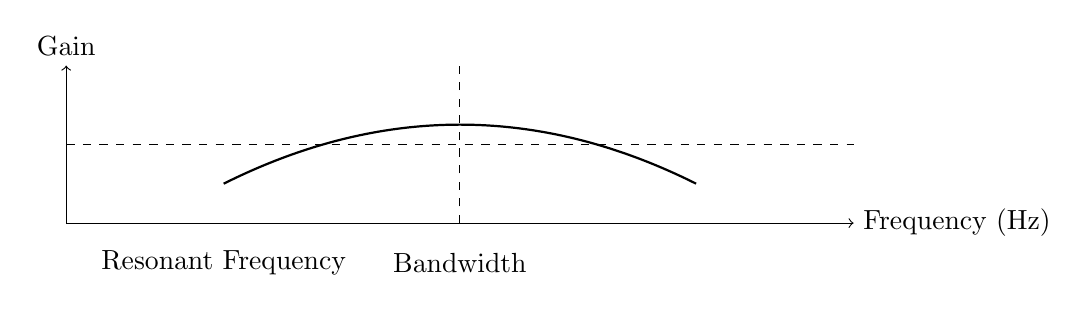
\begin{tikzpicture}
    \draw[->] (0,0) -- (10,0) node[right] {Frequency (Hz)};
    \draw[->] (0,0) -- (0,2) node[above] {Gain};
    \draw[thick] (2,0.5) .. controls (4,1.5) and (6,1.5) .. (8,0.5) node[right] {};
    \draw[dashed] (0,1) -- (10,1);
    \draw[dashed] (5,0) -- (5,2);
    \node at (2, -0.5) {Resonant Frequency};
    \node at (5, -0.5) {Bandwidth};
\end{tikzpicture}
\end{center}
